\documentclass[Afour,sageh,times]{sagej}
% Shared mathematical and layout conventions; the SAGE class is unmodified.
\usepackage{fontspec}
\setmainfont{NimbusRoman-Regular.otf}[BoldFont=NimbusRoman-Bold.otf,ItalicFont=NimbusRoman-Italic.otf,BoldItalicFont=NimbusRoman-BoldItalic.otf]
\setsansfont{NimbusSans-Regular.otf}[BoldFont=NimbusSans-Bold.otf,ItalicFont=NimbusSans-Italic.otf,BoldItalicFont=NimbusSans-BoldItalic.otf]
\setmonofont{DejaVu Sans Mono}[Scale=0.78]
\usepackage{mathtools,tabularx,array,etoolbox}
\usepackage[unicode,colorlinks=true,linkcolor=blue,citecolor=blue,urlcolor=blue]{hyperref}
\urlstyle{same}
\setcounter{secnumdepth}{2}
\setcounter{tocdepth}{2}
\setlength{\emergencystretch}{1em}
\newtheorem{proposition}{Proposition}
\newtheorem{theorem}{Theorem}
\newtheorem{lemma}{Lemma}
\newtheorem{remark}{Remark}
\newcommand{\R}{\mathbb R}
\newcommand{\StageBase}{1c73a580441200d6594e2a2a96374edc1c0e98e6}
\def\journalname{IJRR research manuscript}
\def\volumenumber{Draft}
\def\issuenumber{2026}
\def\volumeyear{2026}
% Remove publication metadata placeholders in the document, not in sagej.cls.
\makeatletter
\patchcmd{\@maketitle}{\hbox{}\volumenumber(\issuenumber):\startpage--\endpage\\}{\hbox{}Unsubmitted manuscript\\}{}{\PackageError{paper}{Title metadata patch failed}{}}
\patchcmd{\@maketitle}{\hbox{}\copyright The Author(s) \volumeyear\\}{\hbox{}Authors to be confirmed\\}{}{\PackageError{paper}{Author metadata patch failed}{}}
\patchcmd{\@maketitle}{\hbox{}Reprints and permission:\\}{\hbox{}Prepared for IJRR\\}{}{\PackageError{paper}{Submission metadata patch failed}{}}
\patchcmd{\@maketitle}{\hbox{}sagepub.co.uk/journalsPermissions.nav\\}{}{}{\PackageError{paper}{Permissions metadata patch failed}{}}
\patchcmd{\@maketitle}{\hbox{}DOI: 10.1177/ToBeAssigned\\}{\hbox{}No DOI assigned\\}{}{\PackageError{paper}{DOI metadata patch failed}{}}
\makeatother

\usepackage{xeCJK}
\setCJKmainfont{Noto Serif CJK SC}
\setCJKsansfont{Noto Sans CJK SC}[ItalicFont={Noto Sans CJK SC},BoldItalicFont={Noto Sans CJK SC Bold}]
\setCJKmonofont{Noto Sans Mono CJK SC}
\renewcommand{\abstractname}{摘要}
\renewcommand{\figurename}{图}
\renewcommand{\tablename}{表}
\renewcommand{\refname}{参考文献}
\renewcommand{\proofname}{证明}
\patchcmd{\abstract}{Abstract}{摘要}{}{\PackageError{paper}{Abstract translation failed}{}}
\patchcmd{\keywords}{Keywords}{关键词}{}{\PackageError{paper}{Keyword translation failed}{}}
\runninghead{三维磁性杆的局部结构与全线圈控制}
\hypersetup{pdftitle={三维磁性杆的局部 Birkhoff 结构与全线圈控制},pdfauthor={作者待补充}}
\title{三维磁性杆的局部 Birkhoff 结构与全线圈控制}
\author{[作者、单位及通讯作者信息待补充]}
\begin{document}
\begin{abstract}
几何积分与学习 Hamiltonian 用于磁驱软体机器人仿真的前提，是其对应同一机械动力学与可实现输入。本文在具有12个配置坐标、位形相关惯性和完整 Biot--Savart 线圈力的三维 Kirchhoff 降阶模型上研究这一接口。通过输运一形式、可计算的局部 Moser 图及相容端点生成函数，分别考察结构匹配与原场逼近。提高输运阶数可以减小连续表示误差，但未必改善总积分误差。固定电流保守分支的非可分中心生成方法显示四阶收敛；光滑反馈与采样受限控制则需要不同的结构判断。全线圈端口的能量求导与虚功一致，而局部仿射场在所测位形上产生约98.6\%的广义力偏差。冻结复网络的比较揭示场精度与动量正曲率之间的取舍。三维共振计算保留了非作用量四次项，尚未建立 KAM 证书。向空间 Cosserat 杆的转移实现了规定血流和接触下的受限执行，但没有改善跟踪。本文建立了力学、结构与磁执行之间可复现且明确局部的连接，并给出当前验证的边界。
\end{abstract}
\keywords{磁驱软体机器人；Cosserat 杆；Birkhoff 系统；几何积分；Hamiltonian 学习；受限磁控制}
\maketitle
\section{引言}
磁驱动能够在细长机器人末端不安装电机的情况下施加力和力矩，但用于血管介入时，形状、材料姿态、周围流体与执行器几何共同决定运动，因而对模型提出了较高要求。本文的长期应用目标是空间站微重力条件下的三维柔性血管内机器人。重力主导载荷减弱，并不意味着血流作用、壁面相互作用、磁工作空间约束或转动惯性消失。本文研究支撑这一目标所需的数学与计算接口；证据来自仿真和局部分析，尚不构成生理或临床验证。

只有先说明保持的是哪一动力学对象的结构，保结构更新才具有明确意义。正则 Hamiltonian 降阶在保守分支上给出一种结构，非保守载荷通常破坏其保持性。时间相关 Birkhoff 形式可以局部表示光滑受载向量场，但近似输运形式可能表示的是邻近向量场。同样，学习得到的标量能量定义了保守预测器，而磁执行器只能施加受限的动量广义力。混淆这些对象，可能在结构缺陷很小的同时产生不准确的物理轨迹。对于具有位形相关质量与空间变化线圈场的三维杆，这一区别尤其重要。

本文以包含两向弯曲和扭转的几何 Kirchhoff 降阶模型研究上述接口，并通过空间 Cosserat 模型考察环境转移。降阶模型保留12个配置变量及质量矩阵的全部导数。完整 Biot--Savart 磁能给出电流到广义力的映射，随后在明确的光滑分支上评估局部一形式输运、Moser 图和端点生成函数。Hamiltonian 学习与共振诊断共用理想偏置保守降阶模型，完整线圈闭环则单独标明。因此，本文给出的是具有明确适用范围的模型接口连接，而不是将所有方法合并为一项实验。

本文成果分为三部分。首先，建立从变惯性杆向量场到输运二形式及相容生成更新的可计算局部连接，分别保留表示、坐标图、积分与求解器误差。推导明确端点横截性、初始规范及固定坐标递推，并在自治保守分支恢复非可分四阶中心方法。这是在既有几何力学框架中的应用与相容条件展开，不将 Darboux 或生成函数理论本身作为本文首创。其次，把磁势、虚功、反馈求导和受限分配连接到同一几何降阶模型，并量化局部仿射场在所测线圈几何中的失效。最后，报告学习、共振与空间杆转移的边界：有限样本上的场预测准确不保证动量曲率为正；形式共振 twist 非零不构成 KAM 证书；端口执行满足约束也不保证跟踪改善。

\section{相关工作及研究记录的适用范围}
几何精确杆模型区分中心线变形与材料标架转动。\citet{Antman2005,Simo1985} 给出其变分与计算基础，\citet{Gazzola2018} 研究柔性细丝的正、逆力学。这些模型支持在完整 Cosserat 计算中保留剪切与伸长，同时在低维解析模型中明确施加 Kirchhoff 约束。\citet{Abbott2020} 综述磁驱动方法及其工作空间依赖性；铁磁连续体机器人展示了相应物理平台 \citep{Kim2019}，受限管腔中的磁软体机器人仿真与导航则为本文参数及实现来源提供参考 \citep{Tong2025}。本文线圈阵列与残余加速度仍是基准设定，而非硬件测量或微重力生理数据。

生成函数可用于构造正则差分格式 \citep{Feng1989}，辛算法的系统理论见 \citet{FengQin2010,Hairer2006}。Birkhoff 格式将结构问题推广到非正则二形式 \citep{Su2007}。对于耗散物理动力学，二形式的时间相容性不可缺少：空间闭性本身不能证明其表示给定向量场。本文通过辅助 Moser 流计算局部坐标图，并保留图的时间导数。原机器人精确流只用于局部存在性论证，不作为可用数值输入。本文四阶格式是适用于非可分 Hamiltonian 的中心生成方法，而非可分系统的漂移--踢步组合。

Hamiltonian 神经网络通过能量的导数定义向量场 \citep{Greydanus2019}。从学习进入 KAM 的论证需要比有限测试损失强得多的范数控制与假设 \citep{Chen2022}。经典与有限可微持久性结果 \citep{Poschel2001,Bounemoura2020}，以及辛算法的离散结果 \citep{Shang1999}，明确了这些证明责任。本文圆截面杆存在四对相等弯曲频率，因此不能直接复用非共振两模态证书。本文将既有有限特征及统计推论保留为条件性结果，报告已计算的共振项，而不宣称得到新的不变环面。

本文证据截止于 Stage~5 分支的仓库提交 \texttt{1c73a58}。原始1025稿件提供物理与数学意图，Stage~4审查指出必要修正，Stage~5提供实现及已有验证。本文不使用 Stage~6 或后续衔接研究的新结果，不新增科学仿真或训练。已有输出按其记录的验证状态选用，被否定的导数计算及失败分配保留独立身份。随附清单把公式、数值主张及图中序列对应到精确源文件与字段。这一范围限制很重要：仓库中历史两模态及平面实验的存在，不能证明新的三维结论。

\section{三维力学与可实现的磁控制}
\label{sec:model-control}

\subsection{同一机器人的两种力学分辨率}
物理对象是残余微重力条件下血管内的柔性磁机器人。仅有中心线不足以确定其状态：中心线保持直线时，材料扭转仍可变化。因此同时保留中心线 $r(s,t)\in\mathbb R^3$ 与材料标架 $R(s,t)\in SO(3)$，其中 $s\in[0,L]$ 为参考弧长。Cosserat 应变与体坐标角速度定义为
\begin{equation}
 \nu=R^Tr_s,\qquad \widehat\kappa=R^TR_s,\qquad
 \widehat\Omega=R^TR_t,
 \label{eq:rod-kinematics}
\end{equation}
其中 $\widehat a b=a\times b$。记内力、内力矩为 $n$、$m$，外力与外力偶密度为 $f,\ell$，则平衡方程为
\begin{equation}
\begin{aligned}
 \rho_s A r_{tt}&=n_s+f,\\
 R\bigl(J_b\dot\Omega+\Omega\times J_b\Omega\bigr)
 &=m_s+r_s\times n+\ell.
\end{aligned}
 \label{eq:rod-balance}
\end{equation}
$J_b$ 是每参考长度的转动惯量。初始直杆采用弹性本构
$n=RK_s(\nu-e_3)$、$m=RK_b\kappa$，其中
$K_b=\operatorname{diag}(EI_1,EI_2,GJ_p)$；$K_s$ 专指剪切/伸长刚度，与 Birkhoff 二形式无关。该约定明确保留双轴弯曲、扭转和转动惯性 \citep{Antman2005,Gazzola2018}。

本文使用目的不同的两种分辨率。空间 Cosserat 模型允许剪切和伸长，计算规定血流、壁面接触、摩擦、磁载荷及残余加速度；基部节点和首个材料标架固定，远端自由。解析模型则施加 Kirchhoff 约束 $\nu=e_3$，在两个弯曲应变与扭转应变中各使用四个归一化 Legendre 基函数。因此，它具有 12 个配置坐标和 24 个相空间坐标。20、40、80 个空间单元仅用于求积，并不增加配置自由度。标架指数更新和中心线中点积分给出实际三维嵌入。两模型共享材料与磁参数，但尚无二者之间的统一误差界。

基准参数为 $L=100$\,mm、半径 $0.6$\,mm、$E=3$\,MPa、$G=1$\,MPa、密度 $1800$\,kg\,m$^{-3}$。远端 $5$\,mm 沿材料轴永久磁化，线磁矩密度为 $0.1448$\,A\,m，总磁矩为 $7.24\times10^{-4}$\,A\,m$^2$。理想轴向偏置场为 $0.5$\,mT。材料和磁化数值是参考文献支持的基准输入 \citep{Tong2025}；沿整根杆使用相同弹性常数是模型假设。密度、阻尼、线圈额定值、壁面参数及残余加速度属于工程或合成设定，并非植入器械实测值。

环境模型中的流体密度、黏度分别为 $1060$\,kg\,m$^{-3}$ 和 $3.5$\,mPa\,s。规定弯管抛物线速度剖面的中心线速度尺度为 $0.04$\,m\,s$^{-1}$，脉动比例为 $0.45$，频率为 $1.2$\,Hz。程序实现各向异性线性相对阻力、含杆直径的横向二次阻力及轴向旋转阻力。量纲一致的 Morison 型惯性扩展应依赖流体加速度与相对加速度；本文未实现附加质量。即使相对阻力耗散，规定流速仍可能向杆输入机械能。管腔壁刚性且静止，标称半径为 $3$\,mm。正穿透量 $\delta_+$ 对应接触势密度 $k\delta_+^{5/2}/(5/2)$，并叠加仅压缩的法向阻尼与正则化切向摩擦。结构阻尼率为 $2$\,s$^{-1}$。残余加速度 $(8,-5,2)\times10^{-5}$\,m\,s$^{-2}$，以及幅值 $3\times10^{-5}$\,m\,s$^{-2}$、标称频率 $3$\,Hz 的抖动，构成合成微重力工况。规定流场与该壁面模型均不构成双向流固耦合。

\subsection{保留完整惯性的正则缩放}
以 $q$ 表示物理 Ritz 系数。几何嵌入给出平移速度和体坐标角速度 Jacobian $J_r(q,s)$、$J_\Omega(q,s)$，从而
\begin{equation}
\begin{aligned}
 M(q)&=\int_0^L\left(\rho_s A J_r^TJ_r+
 J_\Omega^TJ_bJ_\Omega\right)\,ds,\\
 p&=M(q)\dot q.
\end{aligned}
 \label{eq:geometric-mass}
\end{equation}
每次计算均保留位形相关质量。尤其，$\dot p_a$ 中的动能贡献为
$\tfrac12\dot q^T(\partial_{q_a}M)\dot q$；删去该项会改变实际向量场。固定缩放
\begin{equation}
\begin{gathered}
 q=S_qQ,\qquad p=S_pP,\\
 S_q^TS_p=\frac{E_0}{\omega_0}I,\\
 \tau=\omega_0t,\qquad h=H/E_0.
\end{gathered}
 \label{eq:canonical-scaling}
\end{equation}
给出 $z=(Q,P)$、$z'=J\nabla h$，以及
\begin{equation}
\begin{aligned}
 \overline M(Q)&=\frac{\omega_0^2}{E_0}S_q^TM(S_qQ)S_q,\\
 T/E_0&=\tfrac12P^T\overline M(Q)^{-1}P.
\end{aligned}
 \label{eq:scaled-mass}
\end{equation}
撇号表示对 $\tau$ 求导；$J=\left(\begin{smallmatrix}0&I\\-I&0\end{smallmatrix}\right)$。
默认 20 单元模型中，$E_0=3.62\times10^{-7}$\,J，$\omega_0=4.4576294085$\,rad\,s$^{-1}$。缩放由理想偏置场的线性化构造，此后保持固定。它既不保证 $Q=0$ 为全线圈系统的平衡点，也不使理想线性频率成为新线圈平衡的频率。下文状态范数均为无量纲正则坐标范数，具有长度单位的末端误差须由几何重构获得。

理想场分支采用 $h_{\rm ideal}=(T+V_e+V_{\rm uniform})/E_0$，可减去常数零点。全线圈分支则采用
\begin{equation}
\begin{aligned}
 h_{\rm coil}(z,i)&=\tfrac12P^T\overline M^{-1}P\\
 &\quad+V_e(S_qQ)/E_0+\phi(Q)^Ti.
\end{aligned}
 \label{eq:coil-hamiltonian}
\end{equation}
$i\in\mathbb R^{12}$ 为以安培计的总电流。预通电偏置 $i_b$ 拟合局部轴向目标，其最大幅值为 $1.5124804$\,A。式 \eqref{eq:coil-hamiltonian} 不再叠加理想偏置磁势。因此，理想场与线圈分支之间的比较改变了物理势能，而同一分支内积分器的比较保持该势能不变。

\subsection{全线圈能量、虚功与可达性}
工程空芯阵列含十二个半径 $25$\,mm、300 匝的圆线圈，线圈中心到场原点 $(0,0,100)$\,mm 的距离为 $75$\,mm。其几何由归档基准固定，未经硬件标定。对永久磁化和准静态线性线圈场 \citep{Abbott2020}，
\begin{equation}
\begin{aligned}
 B(x,i)&=\sum_{j=1}^{12}b_j(x)i_j,\\
 b_j(x)&=\frac{\mu_0N_c}{4\pi}\oint_{C_j}
 \frac{d\ell\times(x-x')}{|x-x'|^3}.
\end{aligned}
 \label{eq:coil-field}
\end{equation}
\begin{equation}
\begin{aligned}
 V_{\rm coil}&=-\sum_e\mu_e(Q)\cdot B(r_e(Q),i)\\
 &=E_0\phi(Q)^Ti,\\
 G_I(Q)&=-D_Q\phi(Q)^T.
\end{aligned}
 \label{eq:current-port}
\end{equation}
每个圆线圈默认使用 256 个导线求积点。光滑性要求到理想导线的距离为正、几何坐标图有效且质量正定。模型未包含磁滞、涡流、热限制、电路电压动力学或互感。

固定电流对能量求导得到
\begin{equation}
\begin{aligned}
 -\partial_{Q_a}V_{\rm coil}
 &=\sum_e\Bigl[(\partial_{Q_a}\mu_e)\cdot B_e\\
 &\qquad+\mu_e^T(\nabla B_e)\partial_{Q_a}r_e\Bigr].
\end{aligned}
 \label{eq:magnetic-virtual-work}
\end{equation}
两项分别包含力矩功与梯度力功。采用 $(\nabla B)_{ab}=\partial_b B_a$ 时，偶极力和力矩为 $(\nabla B)^T\mu$ 与 $\mu\times B$。电流仅通过 $G_Ii$ 进入动量方程。十二通道因此并不意味着十二个独立广义力，更不意味着可以任意修正 24 维相空间。对期望动量力增量 $d$，不可消除的线性残差为
\begin{equation}
 r_\perp=(I-G_IG_I^\dagger)d.
 \label{eq:unreachable-force}
\end{equation}
它与电流、场约束引入的误差分别报告。数值秩依赖所给奇异值阈值和求积设置。

\subsection{反馈导数与能量计账}
对明确指定的合成比例动量阻尼率 $\gamma$，先定义物理场，再代入反馈：
\begin{equation}
\begin{aligned}
 f(z,i)&=J\partial_z h_{\rm coil}(z,i)\big|_i-
 \binom{0}{\gamma P},\\
 f_{\rm cl}(z)&=f(z,k(z)),\\
 Df_{\rm cl}&=f_z+f_iDk.
\end{aligned}
 \label{eq:physical-feedback}
\end{equation}
直接使用 $J\nabla_z h_{\rm coil}(z,k(z))$ 会引入非物理力项 $J(Dk)^T\phi$。反之，对 $f_{\rm cl}$ 求导时冻结反馈又会漏掉真实链式导数。隐式闭环残差必须在与状态相同的未知中点上计算输入。

记 $h_b=h_{\rm coil}(z,i_b)$、$v=\partial_Ph_b=\overline M^{-1}P$、$y=G_I^Tv$。理想瞬时共点律
\begin{equation}
\begin{aligned}
 i&=i_b-\kappa y,\\
 h_b'&=-\gamma P^T\overline M^{-1}P-\kappa\|y\|^2\leq0.
\end{aligned}
 \label{eq:collocated-power}
\end{equation}
是实际磁端口的功率恒等式。本文选择 $\kappa=0.2/\|G_I(Q_0)\|_2^2=0.1542504562$，其物理输出与增益为
\begin{equation}
\begin{aligned}
 y_{\rm SI}&=E_0\omega_0y,\\
 \kappa_{\rm SI}&=\kappa/(E_0\omega_0)\\
 &=95590.32245\ {\rm A^2/W}.
\end{aligned}
 \label{eq:port-units}
\end{equation}
此换算使同一反馈可转移到空间杆，其单位电流节点力和材料力矩给出
$y_{{\rm SI},j}=\sum_aF_{j,a}\cdot\dot r_a+\sum_eT_{j,e}\cdot\Omega_e$。
杆模型请求 $i_{\rm req}=i_{\rm ff}-\kappa_{\rm SI}y_{\rm SI}$；名义项仍含局部静态顺应度前馈和位置反馈。耗散端口的转移并未消除名义模型误差。式 \eqref{eq:collocated-power} 也不证明保持原二形式、全状态渐近稳定或 KAM 持续性。

当电流随时间变化时，总磁能与机械能具有不同功率预算：
\begin{align}
 h_{\rm coil}'&=\phi^Ti'-\gamma v^TP,\label{eq:total-power}\\
 [(T+V_e)/E_0]'&=v^TG_Ii-\gamma v^TP.
 \label{eq:mechanical-power}
\end{align}
空间环境模型使用机械能预算，并加入流体、耗散接触、残余加速度与结构阻尼功。接触弹性能已计入机械能，不再重复计为外力功。

\subsection{采样分配与电流记忆}
两种受限策略具有不同目标：一种将共点电流请求投影到可行电流集；另一种求解
\begin{equation}
\begin{gathered}
 \min_{i\in\mathcal C(Q,i_{\rm prev})}
 \tfrac12\|G_I(Q)(i-i_b)-d\|^2,\\
 d=\gamma P.
\end{gathered}
 \label{eq:force-allocation}
\end{equation}
以尝试补偿阻尼。可行集包含 $|i_j|\leq2$\,A、
$|i_j-i_{{\rm prev},j}|\leq20\Delta t$\,A，以及采样约束
$\|B\|\leq5$\,mT、$\|\nabla B\|_F\leq0.03$\,T\,m$^{-1}$，其中 $\Delta t$ 以秒计。固定位形下这些约束为凸约束；端口秩亏可能使力分配极小解不唯一。求解器成功标志和独立可行性检查分别记录，不能替代最优性或光滑性证明。

两次更新间的实际电流为
$i(t)=(1-\theta)i_{\rm prev}+\theta i_{\rm target}$，$0\leq\theta\leq1$。
端点约束保证连续幅值界及几乎处处成立的斜率界。凸性还保证分配所用固定空间采样点上的场约束沿电流线段成立，但不能认证所有运动磁点的全部中间时刻，或整个连续血管工作域。杆模型采用带 5\% 裕度的固定管状采样点和 2\,ms 更新；ROM 则在每个 Runge--Kutta 阶段检查实际运动磁点。

投影、采样和电流斜坡改变了执行输入，因此不能直接将理想耗散恒等式赋予任一受限策略。完整采样 ROM 状态为 $(z,i_{\rm prev})\in\mathbb R^{36}$。仅审计其 $24\times24$ 机械子块会遗漏电流记忆。因此，光滑固定电流 Hamiltonian 动力学、光滑共点反馈和受限采样映射需要各自的结构论证。即便所有已记录电流和场样本满足限值，这一区别仍然成立。

\section{输运结构与局部生成映射}
\label{sec:theory}

力学状态采用归一化向量 $z=(Q,P)\in U\subset\mathbb R^{2n}$，时间为 $\tau$，Hamilton 函数为 $h$，步长为 $\eta=\Delta\tau$。杆降阶模型中 $n=12$，但以下构造与这一维数无关。这里 $M$ 表示归一化质量矩阵。工作域取为质量矩阵正定且所述导数存在的开集。所有局部流、辅助流及隐式分支都必须留在指定域内。约定
\begin{equation}
 J=\begin{pmatrix}0&I\\-I&0\end{pmatrix},\qquad K_0=-J,
 \qquad (Da)_{ij}=\partial_{z_j}a_i .
 \label{eq:th-conventions}
\end{equation}
这一约定统一了变分方程和端点构造的符号。几何积分的基本框架见 \citet{FengQin2010,Hairer2006}；这里明确非可分力学模型所需的相容性与可解性条件。

\subsection{具有可测残差的变分表示}
% Source: stage5/proofs/corrected_mathematics.md, section 3, R7--R10; stage4/audit/birkhoff_full_audit.md, section 2; original1025 p1113--p1125, p1180.
令 $\alpha_\tau=a(z,\tau)^T dz$，$\Omega_\tau=d\alpha_\tau$，则
\begin{equation}
 \Omega_\tau=\frac12\sum_{i,j}K_{ij}\,dz_i\wedge dz_j,
 \qquad K=(Da)^T-Da .
 \label{eq:th-form}
\end{equation}
对 $\int(a^T\dot z-B)\,d\tau$ 作固定端点变分并分部积分，得到
\begin{equation}
 \begin{aligned}
 \delta\mathcal A&=\int\delta z^T(K\dot z-\partial_\tau a-\nabla B)\,d\tau,\\
 Kf&=\nabla B+\partial_\tau a .
\end{aligned}
 \label{eq:th-variation}
\end{equation}
因此若引入 $D=-\nabla B-\partial_\tau a$，向量场应为 $-K^{-1}D$。闭性由 $d^2=0$ 得到；$K$ 的可逆性是独立假设。Cartan 恒等式和 $\iota_f\Omega=-(Kf)^Tdz$ 给出
\begin{equation}
 \begin{aligned}
 \partial_\tau\Omega+\mathcal L_f\Omega&=0,\\
 K_\tau+DK[f]+Df^TK+KDf&=0.
\end{aligned}
 \label{eq:th-compatibility}
\end{equation}
于是流满足 $\Phi_{\tau,s}^*\Omega_\tau=\Omega_s$。所保持的是两个时间截面之间的体积 $\Omega_\tau^n/n!$。它通常不同于欧氏相体积：统一动量阻尼使后者收缩，同时保持一个指数加权二形式。

% Source: stage4/audit/birkhoff_full_audit.md, section 3, recurrence (T); stage5/proofs/birkhoff_transport.md, sections 1--2 and 6; stage5/program/transport_native.py, lie_oneform and source_coefficient_function.
对于光滑且局部可逆的流，$\alpha_\tau=(\Phi_{\tau,s}^{-1})^*\alpha_s$ 给出局部存在性构造。相应微分方程与标量为
\begin{equation}
 \begin{aligned}
 \partial_\tau a+\mathcal L_fa&=0,\qquad B=a^Tf,\\
 \mathcal L_fa&=Da\,f+Df^Ta.
\end{aligned}
 \label{eq:th-homogeneous}
\end{equation}
计算有限时间展开不需要预先知道物理精确流。令 $\theta=\tau-s$，写成 $f=\sum_{j\ge0}\theta^j f_j$ 和 $a=\sum_{j\ge0}\theta^j a_j$，其中系数已包含阶乘分母。逐幂比较得到
\begin{equation}
 a_{m+1}=-\frac1{m+1}\sum_{j+k=m}
       \bigl(Da_j f_k+Df_k^Ta_j\bigr).
 \label{eq:th-time-recursion}
\end{equation}
显式时间依赖必须进入 $f_k$。有限个系数不能证明无限级数收敛。

对实际实现的自治力学分支，写成
$h=T+V$，$T=P^TM(Q)^{-1}P/2$，以及 $f=J\nabla h+(0,r)$。取 $a_0=(P,0)$、$\ell=P^Th_P-h=T-V$，直接求导得 $\mathcal L_fa_0=d\ell+(r,0)$。对一个等价的有源方程作截断更为合适：
\begin{equation}
 \begin{aligned}
 a'&=a_0+b,\qquad B'=h+b^Tf,\\
 \partial_\tau a'+\mathcal L_fa'&=d\ell,\\
 b_1&=-(r,0),\\
 b_{j+1}&=-\frac{\mathcal L_fb_j}{j+1}.
\end{aligned}
 \label{eq:th-source}
\end{equation}
这里 $b^{[r_o]}=\sum_{j=1}^{r_o}\theta^jb_j$ 的截断阶数为 $r_o$，与载荷 $r$ 区分。其表示残差严格为
\begin{equation}
 \begin{aligned}
 e_B&=K^{[r_o]}f-\partial_\tau a'^{[r_o]}-\nabla B'^{[r_o]}\\
    &=-\theta^{r_o}\mathcal L_fb_{r_o},\\
 f_a&=f-(K^{[r_o]})^{-1}e_B .
\end{aligned}
 \label{eq:th-source-residual}
\end{equation}
当载荷为零时，所有 $b_j$ 都为零，每个截断阶数均恢复原 Hamilton 系统。标量方程 $\sigma_\tau+f^T\nabla\sigma=\ell$ 通过 $a=a'-d\sigma$、$B=B'+\sigma_\tau$ 将此构造与齐次输运联系起来。规范变换保持表示残差；截断与规范变换一般不可交换。因此这里通过直接截断有源方程本身来改善有限阶近似。

% Source: stage5/proofs/birkhoff_transport.md, sections 3 and 7; stage5/program/transport_cache.py, OneFormCache and CachedRepresentedField; stage5/proofs/high_derivative_ad.md, replacement-path discussion.
数值坐标图在固定中心使用这些一形式系数的空间 Taylor 多项式 $\widetilde b_j$，保留 $h$、$f$、$Df$ 的完整求值器。然而，被表示的场仍发生变化：取 $\widetilde B=h+\widetilde b^Tf$ 和 $\widetilde K=K_0+D\widetilde b^T-D\widetilde b$，则
\begin{equation}
 \begin{aligned}
 \widetilde e_B&=-\bigl(\widetilde b_\tau+D\widetilde b f
                         +Df^T\widetilde b+(r,0)\bigr),\\
 \widetilde f_a&=f-\widetilde K^{-1}\widetilde e_B .
\end{aligned}
 \label{eq:th-cache-residual}
\end{equation}
因此时间截断、系数的空间近似与数值积分各有独立误差。高阶导数使用代数等价表达式 $P^TM(Q)^{-1}P/2+h(Q,0)$ 求值，质量矩阵在当前位形重新计算。独立的反向模式方向导数和有限差分检验所选求导路径；仅有代数等价或张量对称性，不能验证自动微分实现正确。

独立导数检验的必要性可由标量函数 $h(Q,P)=P^2/[2(1+Q^2)]$ 看出。其展开给出 $h_{QQPP}(0)=h_{PPQQ}(0)=-2$。在所检验的软件版本中，一条经过线性求解的混合求导路径将一个四阶分量计算为零。张量指标置换平均一般不能纠正这种错误，因为与同一方向的重复副本收缩时，平均不改变结果。因此，对替代表达式还须数值交叉检查输运系数实际使用的导数量。这些检查提供的是针对所选路径、点和方向的证据。

这一区分直接影响计算解释：即使被表示的向量场与目标场存在明显差异，坐标图积分器仍可准确保持缓存的闭二形式。在缓存中心，精确的系数值和一阶导数可重现原生时间截断残差。离开中心后，须独立计算原生系数才能评估空间近似。小的拉回缺陷或隐式残差均不能界定这一差异。当前构造使用一个固定时间原点和空间域；若通过重叠局部坐标图延拓，还须保证过渡映射和二形式一致。

\subsection{可计算的正则坐标图及其时间导数}
% Source: stage5/proofs/birkhoff_transport.md, section 4; stage5/program/moser_chart.py, auxiliary, map, transformed_field, transformed_jacobian.
在每个固定物理时间，令
\begin{equation}
 \begin{aligned}
 K_{\lambda,\tau}&=K_0+\lambda(\widetilde K_\tau-K_0),\\
 v_{\lambda,\tau}&=K_{\lambda,\tau}^{-1}\widetilde b(\cdot,\tau),\\
 \partial_\lambda\rho_{\lambda,\tau}
     &=v_{\lambda,\tau}\circ\rho_{\lambda,\tau}.
\end{aligned}
 \label{eq:th-moser}
\end{equation}
其中 $\rho_{0,\tau}=\mathrm{id}$。$\widetilde K_\tau$ 的下标 $\tau$ 表示时间截面。此同伦要求每个 $\lambda\in[0,1]$ 都非退化，仅有端点非退化还不够。因为 $\iota_v\Omega_{\lambda,\tau}=-\widetilde b^Tdz$，对拉回求导得 $\rho_{1,\tau}^*\widetilde\Omega_\tau=\Omega_0$。因此 $\chi_\tau=\rho_{1,\tau}^{-1}$ 是正则坐标图。

记 $\rho=\rho_{1,\tau}$、$\mathsf R=D_y\rho$、$\upsilon=\partial_\tau\rho$。正则坐标中的向量场为
\begin{equation}
 u(y,\tau)=\mathsf R^{-1}\{\widetilde f_a(\rho(y,\tau),\tau)-\upsilon\}.
 \label{eq:th-chart-field}
\end{equation}
其中包含坐标图的时间导数。相容性使 $(K_0u)^Tdy$ 闭，因而在星形坐标域内存在局部标量 $\mathcal h$ 使 $u=J\nabla\mathcal h$。辅助求解同时积分 $\mathsf R'=Dv\mathsf R$ 与 $\upsilon'=Dv\upsilon+v_\tau$，初值分别为 $I$、$0$。二阶敏感度 $\mathsf S=D_y^2\rho$ 和 $\mathsf W=D_y\upsilon$ 满足
\begin{equation}
 \begin{aligned}
 \mathsf S'&=Dv\mathsf S+D^2v[\mathsf R,\mathsf R],\\
 \mathsf W'&=Dv\mathsf W+D^2v[\mathsf R,\upsilon]+Dv_\tau\mathsf R,\\
 Du&=\mathsf R^{-1}\{D\widetilde f_a\mathsf R-\mathsf W-\mathsf S[\cdot,u]\}.
 \end{aligned}
 \label{eq:th-chart-sensitivities}
\end{equation}
这些方程给出被表示动力学的完整切线。一个充分的域条件是 $\sup_U\|\widetilde K-K_0\|_2\le\delta_K<1$，于是 $\sigma_{\min}(K_{\lambda,\tau})\ge1-\delta_K$。对 $\|\widetilde b\|/(1-\delta_K)$ 的界进一步控制辅助位移。由浮点系数计算的多项式界可作为该多项式的充分估计，但不是整个物理模型的区间证书。

同伦条件与端点横截性承担不同作用。前者保证整个辅助区间内可构造坐标图；后者保证所选生成坐标能够参数化端点图。即使坐标图准确，也不能保证所有端点投影在较长物理区间内始终正则。因此，数值实现分别检查坐标图匹配、逆复合、坐标图时间导数和隐式切线。辅助求解仅使用缓存一形式及其导数，不通过积分无法获得的精确物理流来构造坐标图。

\subsection{端点相容性与固定坐标生成}
% Source: stage5/proofs/corrected_mathematics.md, sections 4--5, A1--A4 and B1--B4; stage4/audit/birkhoff_full_audit.md, sections 5--6; original1025 p0862--p0888 and p1179--p1213.
\paragraph{定理 A（局部端点生成函数）.}\label{thm:endpoint}
设 $\Omega_s$ 和 $\Omega_\tau$ 分别为两个端点域上的闭非退化二形式。设局部微分同胚 $\Phi$ 满足 $\Phi^*\Omega_\tau=\Omega_s$，局部可逆的端点变换 $\mathcal E:(z_+,z_-)\mapsto(\widehat w,w)$ 满足
\begin{equation}
 \mathcal E^*d(\widehat w^Tdw)=\Omega_\tau(z_+)-\Omega_s(z_-).
 \label{eq:th-endpoint-pullback}
\end{equation}
记 $D\mathcal E=\left(\begin{smallmatrix}A&B_e\\C&D_e\end{smallmatrix}\right)$、$M_\Phi=D\Phi$。若 $CM_\Phi+D_e$ 非奇异，则在充分小的星形 $w$ 域上存在标量 $\phi$，使
\begin{equation}
 \begin{aligned}
 \widehat w&=\nabla_w\phi,\qquad N=\phi_{ww},\\
 N&=(AM_\Phi+B_e)(CM_\Phi+D_e)^{-1}=N^T.
\end{aligned}
 \label{eq:th-endpoint-hessian}
\end{equation}
反之，由 $(z_+,z_-)=\mathcal E^{-1}(\nabla\phi,w)$ 重构端点时，只要负端点投影的导数非奇异，就得到保持二形式的映射。

事实上，将 \eqref{eq:th-endpoint-pullback} 拉回到 $(\Phi(z_-),z_-)$ 使 $\widehat w^Tdw$ 成为闭一形式。横截性使 $w$ 可作坐标，局部 Poincar'e 引理给出 $\phi$。分别对两个端点变量微分即可得到其 Hessian。重构使用联合端点逆；当下式所需分块可逆时，
\begin{equation}
 M_\Phi=(A-NC)^{-1}(ND_e-B_e).
 \label{eq:th-endpoint-reconstruction}
\end{equation}
无需对 $N$ 求逆。在正则中心坐标的恒等映射处，$N=0$，而所需投影仍然可逆。

初始生成函数也必须由此几何结构确定。反解 $w_0(z)=\mathcal E_2(z,z,s,s)$，并令 $c_0(w;s)=\mathcal E_1(z(w),z(w),s,s)$。闭性给出归一化势函数
\begin{equation}
 \phi_0(w;s)=\int_0^1 c_0(w_*+u(w-w_*);s)^T(w-w_*)\,du .
 \label{eq:th-initial-gauge}
\end{equation}
一般而言 $c_0$ 非零。只有指定随时间变化的加性规范后，势函数才唯一。初始横截性仅保证一个局部时间区间；继续延拓要求联合逆和两个投影保持正则。

例如，将正则中心变量改为 $\widehat w=J(y_+-y_-)+\nabla\psi(w)$ 时，因为 $d(\nabla\psi^Tdw)=0$，端点二形式不变。在对角线上得到 $c_0=\nabla\psi$，而不是零，其归一化初始势为 $\psi(w)-\psi(w_*)$。这个例子区分了端点规范的选择自由度和独立的横截条件。采样端点 Jacobian 非奇异仅说明该采样点正则；统一延拓需要邻域界，防止其最小奇异值趋于零。

\paragraph{定理 B（固定 $w$ 的演化与截断）.}\label{thm:fixed-w}
在共同局部解析域上满足定理 A 的假设，令 $g=\nabla_w\phi$、$N=D_wg$。以下量都通过 $(g,w,\tau,s)$ 处的完整端点逆评价：
\begin{equation}
 \begin{aligned}
 \left.\partial_\tau g\right|_w
 &=(A-NC)f(z_+,\tau)\\
 &\quad+\mathcal E_{1,\tau}-N\mathcal E_{2,\tau}\\
 &=:\Psi(g,w,N,\tau;s).
\end{aligned}
 \label{eq:th-fixed-w}
\end{equation}
这由 $\dot{\widehat w}=A f+\mathcal E_{1,\tau}$、$\dot w=Cf+\mathcal E_{2,\tau}$ 和 $\dot{\widehat w}=N\dot w+\partial_\tau g|_w$ 直接得到。对 $g=\sum_{j\ge0}\theta^jc_j$，可计算递推为
\begin{equation}
 \begin{aligned}
 c_{m+1}&=\frac1{m+1}[\theta^m]\Psi\Bigl(
 \sum_{j=0}^m\theta^jc_j,w,\\
 &\hspace{2em}\sum_{j=0}^m\theta^jD_wc_j,s+\theta;s\Bigr).
\end{aligned}
 \label{eq:th-fixed-recursion}
\end{equation}
特别地，$2c_2=(\Psi_\tau+\Psi_g c_1+\Psi_N[D_wc_1])_0$。精确 $N$ 的对称性给出每个 $D_wc_j$ 的对称性。因此每个有限截断仍是标量梯度，只要投影保持正则，就重构出保持二形式的局部映射。局部流的解析依赖和解析端点逆保证局部展开收敛；有限光滑性只能支持相应的有限 Taylor 余项。精度还需要统一的逆映射界及单步稳定性。

对正则端点 $y_\pm$，取 $w=(y_++y_-)/2$、$\widehat w=J(y_+-y_-)$，联合逆为 $y_\pm=w\mp J\nabla\phi/2$。固定标量的时间规范后，\eqref{eq:th-fixed-w} 化为
\begin{equation}
 \begin{aligned}
 \partial_\tau\phi&=-\mathcal h\left(w-\tfrac12J\nabla\phi,\tau\right),\\
 \phi(w,s;s)&=0.
\end{aligned}
 \label{eq:th-central-pde}
\end{equation}
从此标量方程提取系数会自动保持梯度可积性。显式时间依赖通常产生偶次项。已实现的 24 维输运分支是具有时变坐标图的自治光滑场；这些方程不代表已实现任意非自治载荷或接触切换。

具体地，写成 $\phi=\sum_{j\ge1}\theta^j\phi_j$，得到
\begin{equation}
 \begin{aligned}
 \phi_{m+1}&=-\frac1{m+1}[\theta^m]\mathcal h\Bigl(\\
 &\quad w-\tfrac12J\nabla\sum_{j=1}^{m}\theta^j\phi_j,s+\theta\Bigr).
\end{aligned}
 \label{eq:th-scalar-recursion}
\end{equation}
对自治 Hamilton 函数，前几个系数为 $\phi_1=-h$、$\phi_2=0$ 和 $\phi_3=-f^Th''f/24$。这些系数依赖给定 Hamilton 函数的导数，无需未知精确流的值。标量递推还说明，为何不能将自治高阶中心公式直接用于时变正则坐标图：坐标图的显式时间依赖也进入同一系数提取过程。对于所选分支，仍须确认其实现及导数计算成本。

\subsection{力学中点法与非可分四阶映射}
% Source: stage5/proofs/corrected_mathematics.md, section 6, C30--C36; original1025 p0910/m0400 through p1003/m0442; stage3/program/rom_integrators.py, midpoint.
为避免与状态混淆，将原关系式（30）—（34）的端点变量写成 $\widehat\xi=P_+-P_-$、$\widehat\pi=Q_+-Q_-$、$\xi=\overline Q$ 和 $\pi=-\overline P$。其联合逆为 $Q_\pm=\xi\pm\widehat\pi/2$、$P_\pm=-\pi\pm\widehat\xi/2$。对于正则保守场，标量 $-\eta h(\xi,-\pi,\tau_m)$ 生成完整时间中点法。一般有阻尼的物理中点法不会仅因采用这些端点记号就获得标量生成函数。

这一障碍在单自由度中已可见。对于 $\dot Q=P$、$\dot P=-Q-\gamma P$，在 $(\xi,\pi)$ 变量中的候选端点梯度为 $(-\xi+\gamma\pi,-\pi)$。其混合导数分别为 $\gamma$ 和零。阻尼非零时，不存在具有该梯度的局部标量。因此只修正某个阻尼符号不能恢复缺失的相容性。必须先使时变二形式和坐标图表示所选物理场，才能在这些适配坐标中应用端点定理。

对完整变质量系统，修正后的力学方程为
\begin{equation}
 \begin{aligned}
 \delta Q&=\eta M(\overline Q)^{-1}\overline P,\\
 \delta P_i&=\eta\Bigl[-\tfrac12\overline P^T
                  \partial_iM^{-1}(\overline Q)\overline P\\
 &\hspace{3em}-V_{,i}(\overline Q)+r_i(\overline z,\tau_m)\Bigr].
\end{aligned}
 \label{eq:th-mechanical-midpoint}
\end{equation}
质量、几何惯性和反馈均在同一未知中点求值。固定求解器预条件矩阵不改变此残差。仅在质量、刚度 $K_{\mathrm{lin}}$、阻尼 $C_d$ 为常矩阵，且中点力 $F_m$ 预先给定时，消元得到
\begin{equation}
 \begin{aligned}
 E&=\tfrac{\eta^2}{4}K_{\mathrm{lin}}M^{-1}+\tfrac\eta2 C_dM^{-1},\\
 (I+E)P_+&=(I-E)P_- -\eta K_{\mathrm{lin}}Q_-+\eta F_m,\\
 Q_+&=Q_-+\tfrac\eta2 M^{-1}(P_++P_-).
 \end{aligned}
 \label{eq:th-leftsolve}
\end{equation}
这是要求 $I+E$ 非奇异的左线性求解。交换矩阵次序或使用标量除法都会改变方法；依赖状态的中点反馈仍是隐式的。

对光滑的实际闭环场 $f_c$，残差为 $z_+-z_- -\eta f_c(\overline z,\tau_m)$，其导数为 $I-\eta Df_c(\overline z,\tau_m)/2$。因此反馈律必须在未知中点评价，且其状态导数必须进入切线。在所选分支上，残差导数非奇异给出局部可解性。统一压缩映射论证还要求所选域被映回自身；某个计算状态处良好的条件数不能替代这一要求。

% Source: stage5/proofs/integrators_full_coil.md, sections 3--4; stage3/source_inputs/v10/v10_framework_20261028/english/sections/supp_structure.tex, central4 and exact-primitive subsections; stage3/program/rom_integrators.py, central_scalar and central4.
\paragraph{命题（Central4 及其原函数）.}\label{thm:central4}
对自治光滑 Hamilton 函数 $h$，定义 $f=J\nabla h$ 和
\begin{equation}
 \begin{aligned}
 S_\eta&=\eta h+\frac{\eta^3}{24}f^Th''f,\\
 z_+-z_-&=J\nabla S_\eta\bigl((z_++z_-)/2\bigr).
\end{aligned}
 \label{eq:th-central4}
\end{equation}
在光滑单值隐式分支上，若所需导数有界且满足统一局部稳定性，则该对称方法为四阶并恰当辛。不要求动能与势能可分。

为说明修正项，令 $z_c$ 为精确时间中点状态，$m$ 为端点均值。Taylor 展开给出 $m=z_c+\eta^2f'f(z_c)/8+O(\eta^4)$。从端点差中消去 $z_c$，得到
\begin{equation}
 \begin{aligned}
 \delta z&=\eta f(m)+\frac{\eta^3}{24}
          \{f''[f,f]-2(f')^2f\}(m)\\
 &\quad+O(\eta^5).
\end{aligned}
 \label{eq:th-central-expansion}
\end{equation}
记 $A_h=h''$，对 $q_h=f^TA_hf$ 求导得 $\nabla q_h=h^{(3)}[f,f]-2A_hJA_hf$，其 $J$ 倍恰好就是三次修正。因此位形相关质量的混合导数是公式的一部分。这里的正号属于前向中心生成函数修正。

对 $\lambda_0=P^TdQ$，更强的恰当辛恒等式具有明确原函数：
\begin{equation}
 \begin{aligned}
 \Phi_\eta^*\lambda_0-\lambda_0
 &=\overline P^Td(\delta Q)+\delta P^Td\overline Q\\
 &=d\{\overline P^T\delta Q-S_\eta(m)\}.
\end{aligned}
 \label{eq:th-primitive}
\end{equation}
它要求生成函数和隐式分支单值。在具有非零周期的角变量域上，仅有闭性不能给出全局原函数。Cayley 切线 $(I-JS_\eta''/2)^{-1}(I+JS_\eta''/2)$ 描述理想隐式映射；有限迭代残差须单独计入。

统一动量阻尼具有另一种精确结构：对常数 $\gamma$ 与 $r=-\gamma P$，取 $\Pi=e^{\gamma\tau}P$、$\mathcal h=e^{\gamma\tau}h(Q,e^{-\gamma\tau}\Pi)$，得到正则时变系统。其中点更新为 $S_{\eta/2}\circ\mathrm{MP}_{h,\eta}\circ S_{\eta/2}$，这里 $S_a(Q,P)=(Q,e^{-\gamma a}P)$。它在 $D\Phi^TK_0D\Phi$ 中保持因子 $e^{-\gamma\eta}$，并且为二阶。此特例不能将该因子推广到一般阻尼或磁反馈。

\subsection{有条件的有限时间精度}
% Source: stage5/proofs/integrators_full_coil.md, section 5; stage5/proofs/birkhoff_transport.md, section 5; stage3/source_inputs/v10/v10_framework_20261028/english/sections/supp_structure.tex, implicit-solvability subsection.
\paragraph{命题（分离的有限时间缺陷）.}\label{thm:finite-time}
假设在 $[0,T]$ 上存在共同光滑域，坐标图及其逆的导数统一有界，$\|\widetilde f_a-f\|\le\epsilon_f$，且隐式分支稳定。设中点不动点映射将该域内的一个闭凸子集映回自身，并满足 $\eta L/2<1$。若 $\varepsilon_k$ 为代数增量残差，则相减精确与数值中点方程得到
\begin{equation}
 (1-\eta L/2)e_{k+1}\le(1+\eta L/2)e_k+C\eta^3+\|\varepsilon_k\|.
 \label{eq:th-residual-recursion}
\end{equation}
因此积分误差被 $C_T(e_0+\eta^2+\sum_k\|\varepsilon_k\|)$ 控制。Central4 在相应导数与稳定性假设下将 $\eta^2$ 替换为 $\eta^4$。若 $\delta_k$ 界定数值坐标图操作引入的附加状态缺陷，则物理状态误差满足
\begin{equation}
 \begin{aligned}
 \max_{k\eta\le T}\|z_k-z(k\eta)\|
 &\le C_T\bigl(e_0+\eta^p\bigr)\\
 &\quad+C_T\sum_k(\|\varepsilon_k\|+\delta_k)\\
 &\quad+\epsilon_f\frac{e^{LT}-1}{L}.
\end{aligned}
 \label{eq:th-error-bound}
\end{equation}
其中坐标图中点法取 $p=2$，自治保守 Central4 取 $p=4$；当 $L=0$ 时，末项商的取值为 $T$。统一单步残差 $\varepsilon_\eta$ 贡献 $O(\varepsilon_\eta/\eta)$。这同时解释了表示误差平台和固定求解容差下渐近阶数的丧失。逐点坐标图诊断和方向导数检验支持实现，但不认证所有统一假设。此定理仅涉及有限时间，既不提供全局坐标图构造，也不构成新的 KAM 证书。

此误差估计还决定了参考轨迹的比较方式。原场的参考轨迹测量总差异，被表示场的参考轨迹用于分离积分精度。将后者与坐标图更新比较，可测量数值坐标图与中点法的合并贡献。每项比较必须采用相同初态和时间区间。向其中一条参考轨迹收敛，不能替代与另一条参考轨迹的比较。

\section{数值协议与局部输运证据}
\label{sec:numerical}

数值比较明确区分物理向量场、有限阶 Birkhoff 表示以及该表示的数值积分。
所有数值均取自已有冻结输出；制图没有执行新的物理仿真或训练。
共同降阶模型包含12个配置坐标、24个相空间坐标、20个几何单元及配置相关质量矩阵。
完整线圈计算采用12个圆线圈，每圈256个导线求积点。
$z=(Q,P)$ 为缩放正则坐标，$\tau=\omega_0t$，其中
$\omega_0=4.4576294085\,\mathrm{s}^{-1}$。
因此共同时间窗 $T=5\times10^{-4}$ 仅对应 $0.112167$\,ms。
下文状态误差为无量纲欧氏范数，并非毫米单位的末端误差。
能量和功率分别乘 $E_0=3.62\times10^{-7}$\,J 与 $E_0\omega_0$ 转换为 SI 单位。

\subsection{接受的数据来源与比较指标}

最终接受的输运运行名为 \texttt{inverse\_verified}。
高阶求导采用代数等价的完整 $M(Q)$ 逆，并在每个状态重算；物理场和原场参考仍保留原线性求解实现。
独立纯反向求导、有限差分及原生系数比较支持本次具体计算。
早期嵌套前向/反向求解结果，包括 \texttt{synthetic/main.json}，
不作为有效高阶导数证据，原文件继续归档。
程序成功结束本身不能验证导数正确性。
完整线圈范数求导失败及内存失败也保留其原始身份。

对步数 $N\in\{4,8,16\}$、$\eta=T/N$，定义
\begin{equation}
 \begin{aligned}
 E_f(\eta)&=\max_{0\leq j\leq N}\|z_j-z_f(\tau_j)\|_2,\\
 E_a(\eta)&=\max_{0\leq j\leq N}\|z_j-z_a(\tau_j)\|_2.
 \end{aligned}
 \label{eq:numerical-errors}
\end{equation}
其中 $z_f$、$z_a$ 分别为原场与表示场的独立 DOP853 参考。
连续表示误差在65个共同时间点计算。
积分观测阶为 $\log_2[E_a(2\eta)/E_a(\eta)]$；中心场差 $\|f_a-f\|_2$
另作时间喷流诊断。这些最大值均为采样量。
误差范数不能直接标量相加，向量误差抵消可能使 $E_f$ 小于 $E_a$。

合成原场和表示场的两组参考采用
$(\mathrm{rtol},\mathrm{atol},\eta_{\max})=(2\times10^{-10},2\times10^{-12},T/4)$
与 $(5\times10^{-12},5\times10^{-14},T/8)$。
完整线圈输运共享直接积分实验保存的共点分支参考。
后续独立桥接使用当前线圈核重新积分，在65个参考状态上的最大差为 $5.77\times10^{-19}$。
重新拟合偏置电流的最大差为 $6.56\times10^{-14}$\,A，故这里是共同数学反馈定义下，
已量化舍入差的比较，不宣称拟合电流逐位相同。

\subsection{输运阶、积分阶与成本}

合成载荷光滑、状态相关且非比例，不是血流或接触标定模型。
其三阶以内一形式系数的空间次数为 $(2,2,1)$；
完整线圈共点载荷二阶以内的空间次数为 $(2,1)$。
只有这些系数多项式被缓存：原 Hamiltonian、向量场、Jacobian 和完整质量矩阵均在当前状态计算。
两个展开均固定时间原点和缓存中心。

图~\ref{fig:transport} 区分更高输运阶与二阶图中点积分。
在 $\tau=T$，合成分支中心场误差依次为
$3.6233\times10^{-5}$、$6.4510\times10^{-6}$、$1.3243\times10^{-6}$；
连续轨迹差依次为 $8.8402\times10^{-9}$、$1.0556\times10^{-9}$、$1.6462\times10^{-10}$。
但16步原场误差为 $9.6995\times10^{-9}$、$2.0033\times10^{-9}$、$2.2615\times10^{-9}$，
故三阶在本次总误差比较中并非最好。
三个表示场积分的观测阶均约为 $1.9992$。

完整线圈反馈的连续差从 $5.0108\times10^{-8}$ 降至 $1.0785\times10^{-9}$，
最细原场误差从 $5.0169\times10^{-8}$ 降至 $2.4959\times10^{-9}$。
后者仍高于同一原场直接中点的 $2.2449\times10^{-9}$。
这里取得的是可计算的局部表示及其二形式，而不是原场精度全面占优或控制性能已经改善。

辅助 Moser 问题沿自身参数进行数值积分，并非机器人的精确流。
算法传播状态、时间及高阶敏感度，通过反向辅助积分获得逆图。
完整增量残差容差为 $2\times10^{-13}$。
合成分支和完整线圈分支记录的总墙钟时间分别为 $614.900$\,s 和 $1223.641$\,s，
包含系数构造与参考计算。
完整线圈每个网格运行耗时 $44.69$--$116.07$\,s，其中辅助图计算耗时 $0.60$--$1.38$\,s。
这些共享机器上的时间属于实测成本，不构成算法速度排名。

\begin{figure*}[t]
\centering
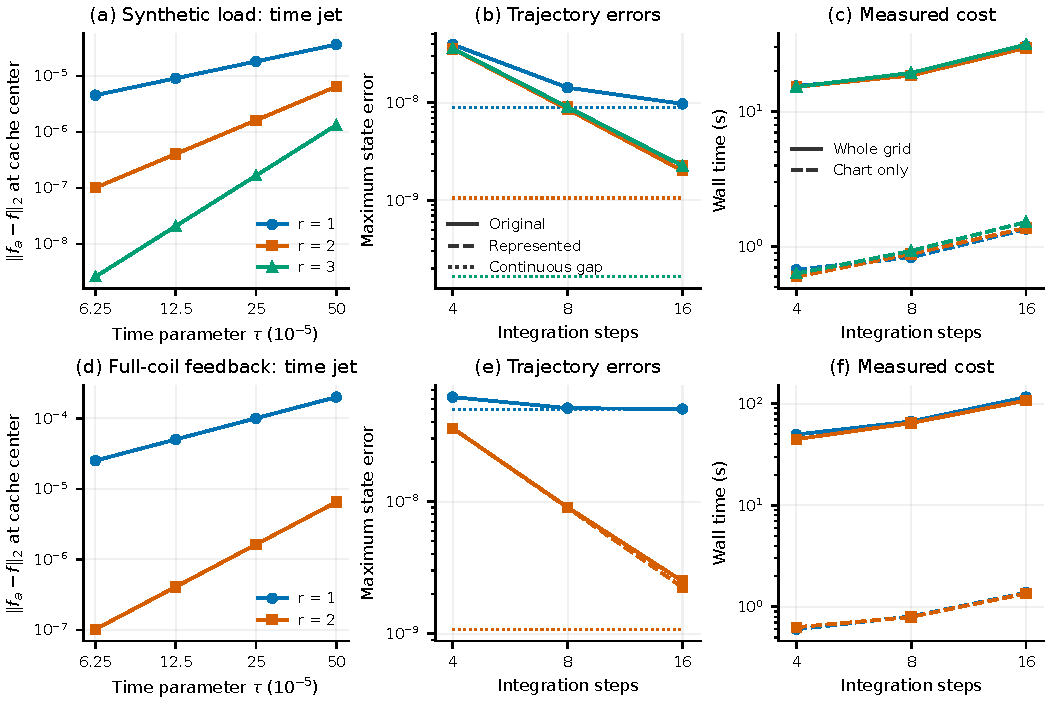
\includegraphics[width=\textwidth]{../figures/transport.pdf}
\caption{最终接受的输运计算。上下两行分别为合成载荷与完整线圈共点反馈。
左：固定缓存中心的原生时间喷流误差。
中：相对原场（实线）与表示场（虚线）的采样轨迹误差，点线为连续参考差；
不同输运阶的表示场误差曲线几乎重合。
右：完整网格墙钟时间与其中辅助图的耗时；系数构造和参考计算不计入这些逐网格时间。
颜色和标记区分输运阶，该阶数不改变中点的二阶时间离散。}
\label{fig:transport}
\end{figure*}

\subsection{直接积分器与失败域}

各直接积分分支分别使用自己的物理场与两组独立 DOP853 参考，设置为
$(2\times10^{-11},2\times10^{-13},T/4)$ 和 $(5\times10^{-13},5\times10^{-15},T/8)$。
固定电流、比例阻尼和共点反馈的参考细化差分别为
$1.24\times10^{-17}$、$8.01\times10^{-18}$、$1.38\times10^{-17}$。
所有方法均从规定的幅值 $0.01$ 初态出发，但只在同一分支内比较误差。
15个方法/网格组合及6组参考总耗时 $690.713$\,s。

固定电流保守分支中，中点与继承的非可分 Central4 最细误差分别为
$2.2449\times10^{-9}$ 和 $1.4749\times10^{-13}$，观测阶分别为 $1.9996$ 和 $3.9966$
（图~\ref{fig:integrators}）。
对合成比例阻尼 $-0.2P$，普通中点与加权中点均为二阶，
但仅加权构造以 $K(\tau)=e^{0.2\tau}K_0$ 为保持目标。
其最细缺陷为 $1.11\times10^{-15}$，普通中点则为 $1.17\times10^{-9}$。
真实共点电流律在未知中点求值，并使用完整反馈 Jacobian。
其正则二形式缺陷为 $3.93\times10^{-4}$：很小的积分残差并不意味着保持 $K_0$。
Central4 和比例加权格式没有被应用于这一一般反馈分支。
结构诊断对全部中点步骤采样理想隐式切映射，而 Central4 仅采样首步；
不宣称浮点程序是精确辛映射。

局部性另有显式测试。
25个时间参数图探测中，合成二阶在 $\tau=0.2$、三阶在 $0.05$ 和 $0.2$，
以及完整线圈二阶在 $0.2$ 时辅助路径越出声明半径 $0.002$，因而被拒绝。
另有两个域外输入按预期拒绝。
这些属于辅助图探测，并非长时间机器人轨迹。
多项式非退化界没有有向舍入，故不是区间证书。
证据支持短时间窗光滑场中的数值连接，尚未建立图间过渡、受限采样反馈结构、
长时间收敛或新的 KAM 证书。

\begin{figure*}[t]
\centering
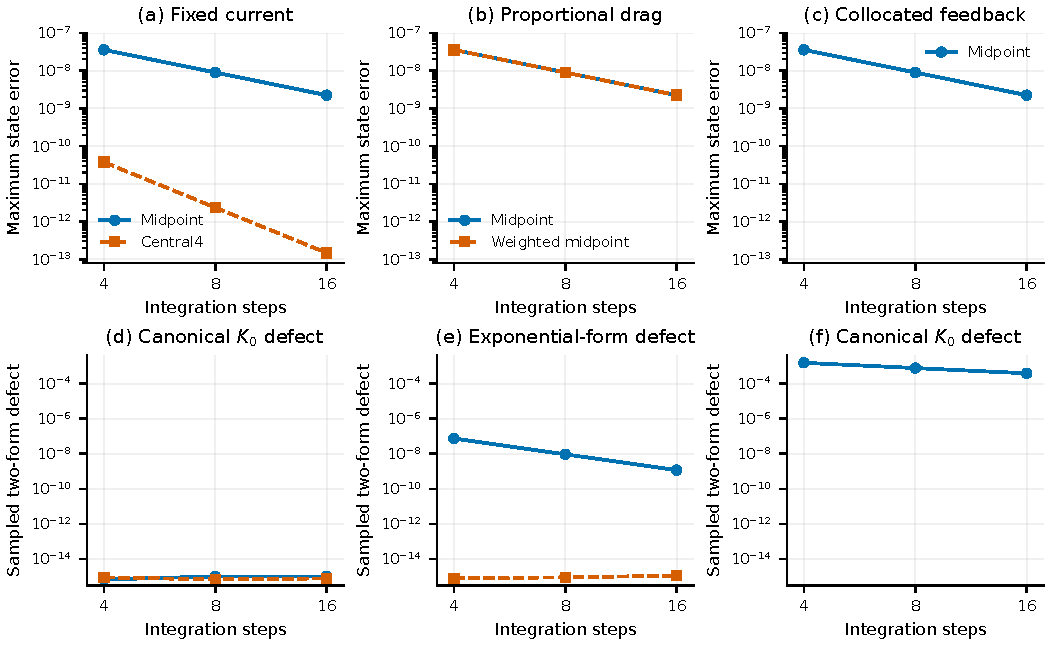
\includegraphics[width=\textwidth]{../figures/integrators.pdf}
\caption{分支内的直接积分比较。
上：相对各自分支精细参考的误差。
下：固定电流与共点反馈的正则二形式缺陷，以及比例阻尼的指数加权二形式缺陷。
比例分支两条误差曲线几乎重合。
缺陷基于理想隐式切映射采样，Central4 仅采样首步。
共点分支非零正则缺陷说明需要针对实际场构造表示，并不否定其二阶轨迹收敛。}
\label{fig:integrators}
\end{figure*}

\section{全线圈验证与空间杆控制转移}
\label{sec:physical-results}

\subsection{能量一致的磁力仍可能否定仿射植物模型}
先对线圈接口进行独立核查，再评价控制。最终线圈核与力分配器中，几何虚功与磁能求导所得力的正则范数差为 $4.44\times10^{-16}$。沿十二个方向、以 $2\times10^{-6}$ 和 $10^{-6}$ 扰动进行能量差分，误差分别为 $3.70\times10^{-10}$ 和 $7.04\times10^{-10}$。圆环轴上场闭式解将绝对 SI 单位核验到 $3.90\times10^{-16}$ 的相对误差；采样散度与旋度缺陷小于 $1.58\times10^{-17}$\,T\,m$^{-1}$。圆线圈求积由 128 加密至 256、512 点，力变化至多 $3.69\times10^{-16}$。这些局部浮点检查支持实现中的能量/力一致性，但不构成连续工作域认证。

尽管如此，全线圈力仍与具有相同原点场、梯度和总电流的仿射场存在显著差异。表~\ref{tab:coil-quadrature} 和图~\ref{fig:coil} 在同一物理 Ritz 系数下比较，并将各网格力统一拉回 20 单元正则坐标。约 98.6\% 的相对差异随空间加密仍然存在，因此不能用导线积分误差或粗网格只有一个磁积分点来解释。相邻空间网格的全力绝对差仍为 $0.00586672$ 和 $0.00145763$，20 单元近似尚未空间收敛。数值秩的增加也表明，应实际测量依赖求积的可达性，而不能从电流通道数推断。

\begin{table}[t]
\centering
\caption{共同位形下的线圈力与可达性诊断。相对力误差为 $\|F_{\rm full}-F_{\rm affine}\|/\|F_{\rm full}\|$；电流端口秩采用相对阈值 $10^{-8}$。}
\label{tab:coil-quadrature}
\begin{tabular}{@{}rrrr@{}}
\toprule
\shortstack{空间\\单元} & \shortstack{磁积分\\点} & \shortstack{相对\\力误差} & \shortstack{$G_I$\\的秩}\\
\midrule
20 & 1 & 0.985235663 & 5\\
40 & 2 & 0.985978752 & 7\\
80 & 4 & 0.986182968 & 7\\
\bottomrule
\end{tabular}
\end{table}

\begin{figure*}[t]
\centering
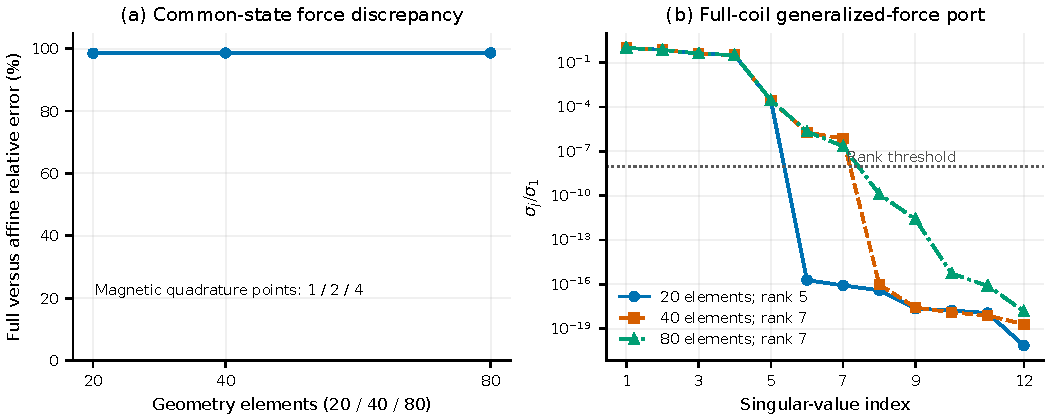
\includegraphics[width=\textwidth]{../figures/coil.pdf}
\caption{20/40/80 个空间求积单元在同一物理 Ritz 系数 $q$ 下的全线圈力差异与电流端口归一化奇异值。所有力和端口均使用共同的 20 单元正则基，磁求积分别有 1/2/4 个有效点。持续存在的约 98.6\% 仿射差异，以及相对阈值 $10^{-8}$ 下 5/7/7 的数值秩，表明不能将十二个线圈通道解释为十二个独立广义力。}
\label{fig:coil}
\end{figure*}

对 $d=0.2P_0$ 和 $0.1$\,ms 分配周期，正交不可达残差为 $2.65530\times10^{-4}$，受限残差为 $4.01583\times10^{-4}$，且 20\,A\,s$^{-1}$ 斜率约束激活。将目标放大 10 倍和 100 倍，受限残差分别为 $0.00500641$ 和 $0.07305644$。正确反馈导数的方向有限差分误差为 $2.40\times10^{-9}$；改为对复合 Hamiltonian 求导会造成 $5.47301$ 的场差，而冻结反馈会漏掉谱范数为 $12.56491$ 的 Jacobian 项。这是两个不同的实现错误，均直接影响隐式闭环更新。

\subsection{实际受限轨迹及其分辨率限制}
受控轨迹由相同 $z_0=\operatorname{initial\_state}(0.01)$、总偏置、材料、增益和约束独立积分得到。取 $\gamma=0.2$，八次控制更新覆盖 $\tau\in[0,0.004]$，即 $0.89733794$\,ms。每周期使用一个或两个 RK4 子步，形成 8 步和 16 步网格。各分支分别计算自身反馈与实际植物力，没有将仿射轨迹复用为全场轨迹。

全植物/全控制器与仿射植物/仿射控制器的最大正则状态范数差为 $3.90705\times10^{-4}$，各自粗细网格差约 $7.22\times10^{-8}$，因此植物近似对轨迹的影响得到分辨。但在同一全植物上，将全场控制器换成仿射控制器仅造成 $7.17555\times10^{-8}$ 的轨迹差。该窗口未分辨出全场控制设计的性能优势。含力补偿在内的四个分支，在细网格上的总能量和机械能--功残差幅值均约为 $6.25\times10^{-11}$。磁点采样场与梯度最大值分别为 $0.501325$\,mT 和 $0.00431404$\,T\,m$^{-1}$。力补偿达到 20\,A\,s$^{-1}$，但仍留下约 $4.01416\times10^{-4}$ 的最大力残差。

最终分配器从经独立验证可行的上一电流启动力目标优化。真实重跑相较此前成功的补偿轨迹，状态最大差为 $1.17\times10^{-12}$，电流最大差为 $6.51\times10^{-10}$\,A。该一致性并不证明优化算法具有相同导数。严格匹配初始偏置后重新计算的 36 维采样映射，共点投影与力补偿的数值秩分别为 28 和 36，在所用正则/电流坐标中的条件数分别为 $5.43\times10^{18}$ 和 $2.09\times10^5$。机械子块相对于 $K_0$ 的缺陷分别为 $3.22749\times10^{-3}$ 和 $1.03008\times10^{-4}$。尽管机械终态差仅 $1.04\times10^{-14}$，新旧力分配 Jacobian 的谱范数差仍为 $1.77112\times10^{-4}$，主要来自电流输出块。因此，可行分配成功和轨迹几乎相同，并不证明采样映射光滑、可逆或辛。

\subsection{环境模型转移：执行可行但跟踪未改善}
\begin{figure*}[t]
\centering
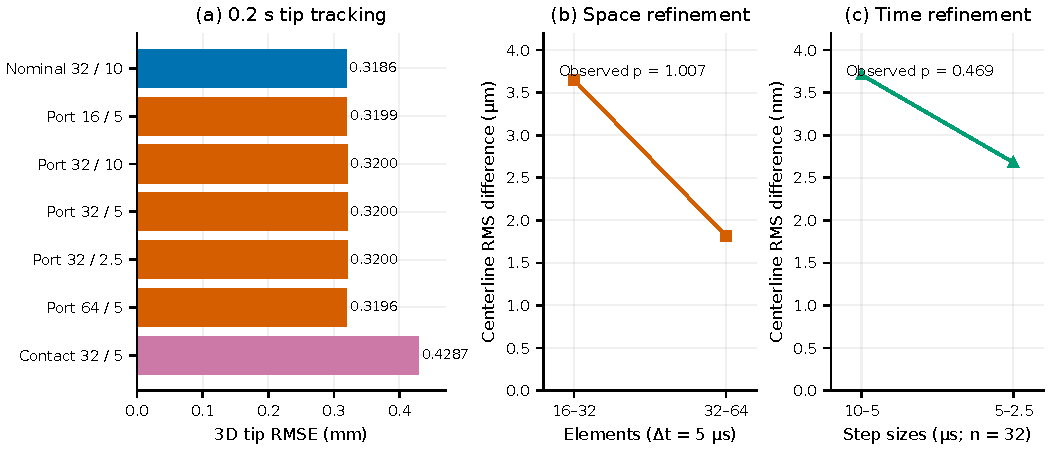
\includegraphics[width=\textwidth]{../figures/rod.pdf}
\caption{空间杆在 0.2\,s 内的控制转移。(a) 标签依次给出单元数和以微秒计的步长；名义控制与端口控制的公平比较采用 32 单元、10\,$\mu$s。接触算例使用独立的 1.6\,mm 半径管腔几何，其余算例采用标称 3\,mm 管腔。(b,c) 为共同输出时刻、129 个参考弧长点上的相邻中心线差异。观察阶描述这些数值差异，并不建立精确 PDE 误差或时间二阶收敛。}
\label{fig:rod}
\end{figure*}
七个空间杆算例采用全线圈力和式 \eqref{eq:port-units} 的物理增益，从直杆静止状态及零实际电流开始积分 $0.2$\,s。此时 $0.3$\,s 的目标斜坡仍未完成。程序使用 PyElastica PositionVerlet，并加入上述环境载荷。相同的 32 单元、10\,$\mu$s 网格上，名义控制末端 RMSE 为 $0.318558$\,mm，加入端口反馈后为 $0.320032$\,mm，跟踪略有恶化。32 单元、5\,$\mu$s 端口算例的 RMSE 为 $0.320033$\,mm，最大电流为 $1.67831$\,A，最大斜率为 20\,A\,s$^{-1}$，电流斜坡连接缺陷为零，387 个固定约束采样点上的已记录违例为零。保存节点的全场和梯度最大值分别为 $0.279966$\,mT 和 $0.0223521$\,T\,m$^{-1}$。这些有限样本不构成连续工作域认证。

标称 3\,mm 管腔未激活接触。独立的 1.6\,mm 半径窄管算例初始无穿透，在运动中产生 $61.6032$\,$\mu$m 的最大穿透和 $11.3524$\,$\mu$N 的总法向力，RMSE 为 $0.428689$\,mm。图~\ref{fig:rod} 单独报告这一应力工况。理想端口增量功率非正，但投影后与斜坡起点的增量功率分别达到正值 $3.19262\times10^{-8}$ 和 $3.20376\times10^{-8}$\,W。32 单元、5\,$\mu$s 算例的机械能--功残差为 $1.24636\times10^{-14}$\,J。因此，准确功率计账与实际执行输入失去理想耗散保证可以同时出现。

原分配器的回退曾引入约 $0.133$\,A 的电流差并破坏时间加密结果。最终程序先截到电流盒，再沿上一可行电流出发的线段解析修复，同时保留所有优化器未收敛状态。七个最终算例均无回退、各有 99 次修复及一至四次未收敛状态，故未将可行性等同于已证最优性。在 129 个共同参考弧长点，相邻中心线 RMS 差对 16/32/64 单元为 $3.64802/1.81514$\,$\mu$m，对 10/5/2.5\,$\mu$s 步长为 $3.70928/2.67939$\,nm。观察空间阶与时间阶分别为 $1.00703$ 和 $0.469234$；这些结果既不提供精确 PDE 误差，也未证实时间二阶收敛。

最后，另设 2\,ms 保守比较，匹配初态、材料和固定电流，并同时关闭流体、管壁、重力与阻尼。ROM 与 16/32/64 单元杆的中心线 RMS 差依次增大为 $7.85933$、$11.2030$、$14.1690$\,nm，末端 RMS 差分别为 $33.4755$、$65.6852$、$86.4209$\,nm。Ritz 截断、剪切/伸长约束、求积及基部标架离散仍构成不同模型误差。该固定电流还在全杆上产生 $0.798394$\,T\,m$^{-1}$ 的梯度，超过 $0.03$\,T\,m$^{-1}$ 限值。因此该诊断不是可行导航结果，也不是已收敛的 ROM 误差证书。

\section{Hamiltonian 学习与共振分析}
\label{sec:learning-kam}

\subsection{具有复可训练表示的实能量}
Hamiltonian 学习通过对标量能量求导获得保守向量场\citep{Greydanus2019,Chen2022}。本节的目标为具有理想均匀轴向磁偏置的变质量 Kirchhoff 模型，记为 $H_{\mathrm{ideal}}$；该模型有 12 个配置自由度、24 维相空间和 20 个几何积分单元。完整线圈系统采用另一磁势。这些保守标签不含流体、接触和阻尼力。因此，学习实验检验的是所声明机械能量的近似，而部署还需要物理端口接口。

采用无量纲正则状态 $z=(Q,P)$、能量 $h=H/E_0$ 和时间 $\tau=\omega_0t$。在物理正则缩放之后定义
\begin{equation}
 \begin{aligned}
 \xi&=(Q+iP)/\sqrt2,\\
 \chi&=(Q-iP)/\sqrt2.
 \end{aligned}
 \label{eq:learn-complex-coordinate}
\end{equation}
实切片上 $\chi=\bar\xi$，全纯延拓时二者独立。逆变换给出
\begin{equation}
 \begin{aligned}
 \partial_\chi&=(\partial_Q+i\partial_P)/\sqrt2,\\
 \{\xi_j,\chi_k\}&=-i\delta_{jk},\\
 \xi'&=-ih_\chi+iR/\sqrt2,
 \end{aligned}
 \label{eq:learn-complex-field}
\end{equation}
其中 $R$ 作用于动量方程。训练损失与预测器必须采用同一导数约定。复参数不会使物理能量成为复值函数，仅设置能量虚部输出也不能实现物理 Rayleigh 阻尼。

训练采用 $x=Dz$，其中 $D=\operatorname{diag}(\sqrt\nu,\sqrt\nu)/a$、$\nu=\omega/\omega_0$、$a=0.08$。这一附加缩放不是正则变换：$\nabla_zh=D\nabla_xh$，且 $x'=DJD\nabla_xh$。所有模型均增加残差 $r_\theta$，其基底为同一二次先验 $h_2=a^2\|x\|^2/2$。

有限解析模型包含动量次数为零或二的全部三次、四次机械残差：$Q^3$、$Q^4$、$QP^2$ 和 $Q^2P^2$，分别贡献 364、1365、936 和 6084 个系数。这 8749 个实参数描述所声明的机械函数类，而非 24 变量的全部四次多项式。完整复网络具有两个宽度为 48 的复隐藏层和一个复读出，共 3552 个复参数，即 7104 个实参数。网络同时使用复输入及其共轭、分离激活 $\sigma(u)=\tanh(\operatorname{Re}u)+i\tanh(\operatorname{Im}u)$、三次门控及 $P\mapsto-P$ 平均。所有权重的实部和虚部均参与训练。门控保留二次先验，平均保留动量偶性；二者均不保证关于动量的凸性。

机械复网络使用 13440 个实参数，预测下三角矩阵 $L(Q)$ 及势能残差；矩阵具有正指数对角元并满足 $L(0)=I$。其能量为
\begin{equation}
 \begin{aligned}
 h_\theta&=\tfrac12a^2x_P^TLL^Tx_P\\
 &\quad+\tfrac12a^2\|x_Q\|^2+V_\theta(x_Q),\\
 (h_\theta)_{PP}&=D_\nu LL^TD_\nu,
 \end{aligned}
 \label{eq:learn-spd}
\end{equation}
其中 $D_\nu=\operatorname{diag}\sqrt\nu$。对有限实输出，有 $v^T(h_\theta)_{PP}v=\|L^TD_\nu v\|^2>0$，对任意 $v\ne0$ 均成立。因此在精确算术下，固定 $Q$ 的动量到速度映射是线性双射。这证明了结构性质，但未给出统一条件数或物理质量误差界。

分离激活是实解析的，但并非单复变量全纯函数。合法延拓将共轭输入替换为独立变量，并使用
\begin{equation}
 \begin{aligned}
 \sigma^{\mathbb C}(u,v)&=\tanh((u+v)/2)\\
 &\quad+i\tanh((u-v)/(2i)),
 \end{aligned}
 \label{eq:learn-analytic-extension}
\end{equation}
同时冻结训练系数及其共轭。这样在避开所有层极点的域内得到局部全纯延拓。所报告的训练并未认证统一极点裕量或复域近似范数。

\subsection{冻结训练与机械诊断}
实验以数据种子 51001 在 $[-1,1]^{24}$ 内均匀抽取 1024 个训练状态和 256 个验证状态。每种架构分别采用种子 51001--51003，进行 1200 次 Adam 更新，批量大小为 128。多项式与网络的学习率分别为 $10^{-3}$ 和 $3\times10^{-3}$，梯度裁剪阈值为 10。令 $r_*=h_{\mathrm{ideal}}-h_2$，实际目标函数为
\begin{equation}
 \begin{aligned}
 \mathcal L&=\operatorname{mean}\left[\left(\frac{D(\nabla_xr_\theta-\nabla_xr_*)}{s_g}\right)^2\right]\\
 &\quad+0.15\operatorname{mean}\left[\left(\frac{r_\theta-r_*}{s_h}\right)^2\right],
 \end{aligned}
 \label{eq:learn-objective}
\end{equation}
其中 $s_h=0.00954395736$ 为训练残差能量标准差，$s_g=0.4661470702$ 为其正则梯度均方根。验证集每 50 次更新选择检查点，同时检查第一次更新。九组权重全部冻结之后，才以种子 510990 生成 $[-1,1]^{24}$ 内的 512 个独立测试标签和 $[-1.5,1.5]^{24}$ 内的 256 个扩展域标签。计算采用 float64/complex128、单 CPU 线程和 PyTorch 2.5.1；记录的本次运行耗时约 410.8\,s。

表~\ref{tab:learn-errors} 和图~\ref{fig:learning} 报告各样本集上的正则场相对 $L^2$ 误差 $\|J\nabla(h_\theta-h_*)\|_2/\|J\nabla h_*\|_2$。在本预算下，无约束复网络精度最高，而仅 SPD 模型保证正动量曲率。二次先验的测试误差为 63.094\%，较小的历史 48 特征读出为 62.964\%。参数数量、函数类、学习率与每次更新成本不同，因此这些比较不能单独识别复参数化相对实参数化的优势。尤其是，有限预算 Adam 并不证明已达到多项式类的最小二乘最优解。

\begin{table*}[t]
 \centering
 \caption{冻结学习结果：三个种子的范围。最后一列为每个种子在八个预先指定测试状态上的非正动量 Hessian 数量。扩展域使用放大 1.5 倍的坐标盒。}
 \label{tab:learn-errors}
 \small\setlength{\tabcolsep}{3.5pt}
 \begin{tabular}{lrrrr}
 \toprule
 模型 & 实参数数 & 测试场误差 (\%) & 扩展域误差 (\%) & 非正 $h_{PP}$ \\
 \midrule
 机械多项式 & 8749 & 35.249--35.282 & 59.743--60.273 & 4/4/4 \\
 完整复隐藏层 & 7104 & 3.241--3.700 & 8.410--9.063 & 2/2/4 \\
 SPD 机械复网络 & 13440 & 11.415--11.553 & 20.651--21.917 & 0/0/0 \\
 \bottomrule
 \end{tabular}
\end{table*}

对每个种子的八个测试状态与八个扩展域状态，分别检查 Hessian、能量二阶差分及 Legendre 方程 $\partial_Ph_\theta(Q,\widehat P)=\partial_Ph_*(Q,P)$。以真实 $P$ 初始化使其成为有利的局部检验。方程残差很小仍可伴随较大的恢复动量误差。部分求解器进展标志为假，但残差已接近舍入量级；无约束复模型还存在实质非零的反解残差。其测试样本中最大的 Hessian 条件数达到 $1.67\times10^5$。SPD 模型扩展域样本的条件数最大约为 1811；正定性不等于惯量准确。多项式、复网络和 SPD 模型的测试样本最大 Hessian 相对误差依次为 47.49\%、5.82\% 和 17.05\%，最大相对恢复动量误差依次为 27.30、0.6267 和 0.5044。独立重新生成的标签和方向二阶差分确认了保存的负曲率符号。

部署所需的学习场修正为 $(-\delta g_P,+\delta g_Q)$，其中 $\delta g=\nabla h_\theta-\nabla h_*$。线圈电流仅直接改变动量方程。因此，独立的受限分配测试 $\delta g_Q$ 的可达部分，同时保留配置速度误差和线圈像空间外的力分量。三个模型、三个种子和八个状态的全部 72 项修正分配均完成；在相对阈值 $10^{-8}$ 下，端口有效秩为五，部分电流达到 2\,A 边界。多项式、复网络和 SPD 模型修正后与修正前的总场误差比依次为 0.8845--0.9898、0.8959--0.9960 和 0.8482--0.9965。该实验是在声明的 0.25\,s 电流变化窗口下进行的静态分配诊断，没有积分学习闭环。


\begin{figure*}[t]
\centering
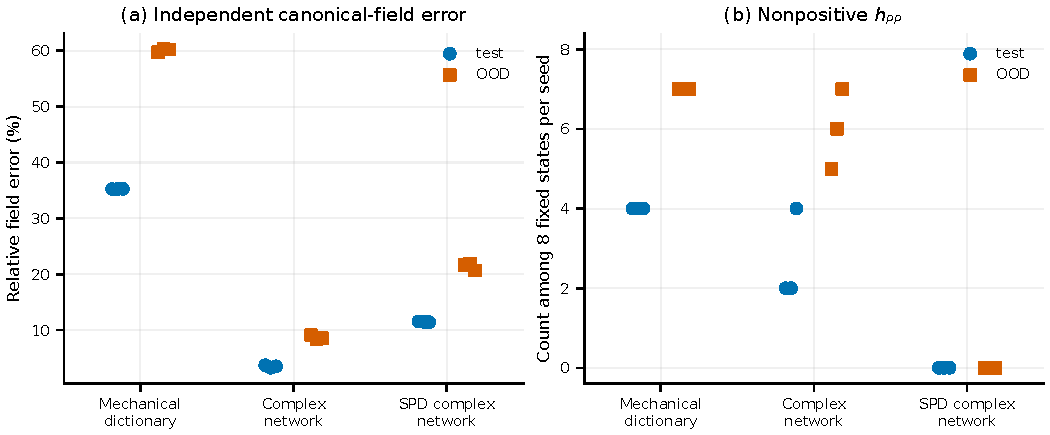
\includegraphics[width=\textwidth]{../figures/learning.pdf}
\caption{冻结 Hamiltonian 学习比较。每个点对应三个训练种子之一；左图为独立测试域及域外的正则向量场误差，右图为每个种子在各数据分区的八个预定状态中非正动量 Hessian 的数量。这些有限样本不构成统一域界。所有模型均针对理想偏置 Hamiltonian 训练，而非完整线圈磁势。}
\label{fig:learning}
\end{figure*}

\subsection{从经验误差到持久性假设}
两条不同的误差论证保留学习与动力学之间的联系。对有限基，写作 $h_\theta=h_0+\sum c_{\theta j}\psi_j$、$h_*=h_0+\sum c_{*j}\psi_j+R$。将样本导数特征堆叠成 $A$，去除常数规范，并对所有残差采用同一观测归一化 $N_o$。若 $G=A^TA/N_o\succeq\lambda I$，则
\begin{equation}
 \begin{aligned}
 \|h_\theta-h_*\|_{\mathcal X}
 &\le B_{\mathcal X}\frac{r+e}{\sqrt\lambda}+\|R\|_{\mathcal X},\\
 B_{\mathcal X}&=\Big(\sum_j\|\psi_j\|_{\mathcal X}^2\Big)^{1/2}.
 \end{aligned}
 \label{eq:learn-gram-bound}
\end{equation}
其中 $r$ 是拟合观测残差，$e$ 包含观测误差与 $R$ 的样本导数。证明只使用最小奇异值与 Cauchy--Schwarz 不等式，不要求样本独立或拟合达到最优。范数可以是实域 $C^\ell$ 范数，也可以是指定复域上的解析上确界范数。积分观测需计入端点与求积误差，导出系数需计入舍入界。旧两模态完整余弦模型保留全部 35 个四次方向，由一个余弦系数和 34 个正交多项式方向实现。其 Gram 下界不能移用于新的 8749 特征字典。

另一条条件性论证\citep{Chen2022}结合参数覆盖、Hoeffding 集中、Poincar\'e 不等式和插值。设 $\mathcal D=\mathbb T^n\times B$、$d=2n$、$p>d$、$\ell\ge1$，且整数 $s>\ell+d/p$。要求独立样本的密度至少为 $m_0$、实化参数位于有界立方体、梯度残差和参数 Lipschitz 常数具有统一界，且固定规范后存在统一 $W^{s,p}$ 界 $M_s$。则以至少 $1-\delta$ 的概率，对整个函数类同时成立
\begin{equation}
 \begin{aligned}
 \|e_\theta\|_{C^\ell}&\le E_\theta,\\
 E_\theta&=C_{\mathrm{GN}}(G_\theta+M_s^\alpha G_\theta^{1-\alpha}),\\
 \alpha&=\frac{\ell-1+d/p}{s-1},
 \end{aligned}
 \label{eq:learn-statistical-bound}
\end{equation}
其中 $G_\theta=C_Pm_0^{-1/p}(\widehat R_\theta+\Gamma)^{1/p}$，$\Gamma$ 是补充材料推导的显式覆盖惩罚。这是统一统计蕴含，而非 Adam 收敛定理。对当前网络，两条论证所需的常数均未全部认证。有限样本梯度误差本身不能补足这些常数：仅在单个标量变量 $w$ 中，多项式 $c\prod_j(w-w_j)^2$ 就能在样本点保持函数值和一阶导数为零，而复域范数可随 $c$ 任意增大。

\begin{figure*}[t]
\centering
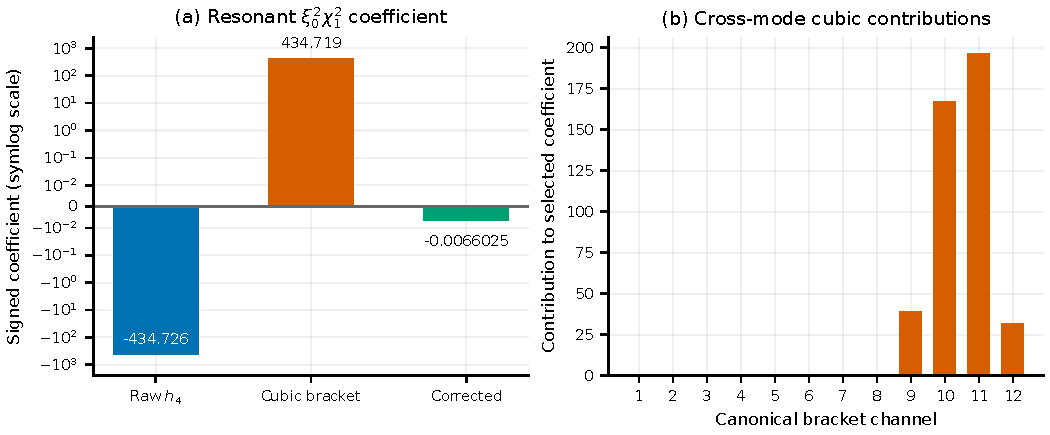
\includegraphics[width=\textwidth]{../figures/resonance.pdf}
\caption{第一频率对四次共振诊断。左图以对称对数尺度显示原四次系数、保留全部12个括号通道的三次消去修正及其较小残差；右图为四个外部扭转括号通道对三次消去修正的贡献，通道从一开始编号。计算保留了全部12个正则通道。原第一频率对子空间并不不变，因此这一受限系数不能证明完整系统的 KAM 非退化性。}
\label{fig:resonance}
\end{figure*}

\subsection{共振的三维机械模型}
实际理想偏置模型的线性化具有四对 $1{:}1$ 弯曲频率，其频率比分别为 $1$、$6.21276315$、$17.89814255$ 和 $80.07400435$。在阈值 $10^{-10}$ 下，全部 2600 个三次单项式中无共振，最小除数为一；17550 个四次单项式中有 206 个位于同调核，包括 78 个作用量项和 128 个非作用量项。成对简并来自圆杆的轴向对称性；数值阈值只是有限阶诊断。

对 $h=h_2+h_3+h_4+\cdots$、$h_2=\sum_j\nu_j\xi_j\chi_j$，同调方程及其三次解为
\begin{equation}
 \begin{aligned}
 \{h_2,\xi^\alpha\chi^\beta\}
 &=i\nu\cdot(\alpha-\beta)\xi^\alpha\chi^\beta,\\
 (W_3)_{\alpha\beta}&=\frac{i(h_3)_{\alpha\beta}}{\nu\cdot(\alpha-\beta)}.
 \end{aligned}
 \label{eq:learn-homological}
\end{equation}
于是 $\{h_2,W_3\}=-h_3$，Lie 展开给出共振四次项
\begin{equation}
 Z_4=\Pi_{\mathrm{res}}\left(h_4+\tfrac12\{h_3,W_3\}\right).
 \label{eq:learn-resonant-quartic}
\end{equation}
限制到第一对弯曲模态时，仍保留全部 12 个正则括号通道。对完整梯度沿选定四个实坐标求两次导数，即可获得在一次求导后仍能对该限制贡献的所有三次单项式；含两个外部变量的项不能贡献。四个外部扭转通道为 $\xi_0^2\chi_1^2$ 系数提供非零修正：
\begin{equation}
 \begin{aligned}
 &-434.7256304212535+434.719027922014\\
 &\qquad\simeq-0.006602499239534154.
 \end{aligned}
 \label{eq:learn-cancellation}
\end{equation}
该抵消超过四个数量级（图~\ref{fig:resonance}）。采用的计算使用反向自动微分，四阶置换缺陷为 $2.27\times10^{-13}$，并通过独立标量求导检查。其原始系数与半径外推之差为 $7.26\times10^{-7}$。先前混合模式导数张量未通过置换对称性检验（缺陷为 1738.9），因此未采用；失败文件仍保留。这些检查验证有限阶数值一致性，没有界定解析尾项或抵消过程中的舍入误差。

计算所得限制满足下式，系数缺陷为 $1.23\times10^{-13}$：
\begin{equation}
 \begin{aligned}
 Z_{4,\mathrm{pair}}&=A(I_0+I_1)^2+BL^2,\\
 L&=Q_0P_1-Q_1P_0,
 \end{aligned}
 \label{eq:learn-pair-form}
\end{equation}
其中 $I_j=\xi_j\chi_j$、$A=0.0004112209869572539$、$B=0.006602499239534154$。酉变换 $\xi_\pm=(\xi_0\mp i\xi_1)/\sqrt2$ 的实化是辛变换，其作用量为 $I_\pm=(N\pm L)/2$，$N=I_0+I_1$。因此形式扭转的特征值为 $4A\simeq0.00164488$、$4B\simeq0.0264100$，行列式为 $16AB\simeq4.34414\times10^{-5}$。32 个状态上的独立检查给出最大作用量恒等式误差 $8.67\times10^{-19}$。然而，原第一对坐标子空间中三个状态的外模态场范数为 0.01643、0.06573 和 0.26300。该子空间不由完整非线性动力学保持。因此，该计算建立的是受限四次候选，而非两自由度物理子系统或全维扭转。一个轴向 $SO(2)$ 动量也不能提供四个独立对称约化；正则约化要求自由作用和正则动量水平，而直杆平衡点不满足这些条件。




\subsection{连续与离散 KAM 的范围}
连续持久性要求：指定正则域上的保守 Hamiltonian、频率映射具有有界逆的可积主部、足够正则性、边界裕量、Diophantine 界 $|k\cdot\omega|\ge\gamma|k|^{-\tau}$（对所有 $k\ne0$ 成立），以及所选定理的小量阈值\citep{Poschel2001}。若同一图上 $h_*=h_0+P_*$、$h_\theta=h_0+P_\theta$，则固定规范后学习扰动的认证界 $\beta_\theta$ 与误差界 $E_\theta$，须在相应定理假设下共同满足 $\beta_\theta+E_\theta<c_K\gamma^2$。分别应用定理可得两套环面族，并不意味着嵌入相同。物理扰动和正规形余项仍属于该预算。

离散持久性还要求在保留域上的解析 exact-symplectic 映射及其逆、周期生成函数、离散扭转和频率裕量，以及
\begin{equation}
 |e^{i\Delta k\cdot\omega}-1|\ge\Delta\gamma_D|k|^{-\tau_D}\quad(k\ne0).
 \label{eq:learn-discrete-divisor}
\end{equation}
生成函数扰动须除以 $\Delta$ 后再与 Hamiltonian 界比较\citep{Shang1999}。小步长本身不能排除 $\Delta k\cdot\omega=2\pi m$。精确隐式方程的辛性也不意味着有限容差求解器就是 exact-symplectic 映射。继承的有限幅值证书针对某个冻结的两模态 Hamiltonian，使用其自身 Fourier 候选和验证域计算；它不为当前任一种三维磁势提供证书。这里尚未认证完整共振耦合、扭转逆、域与余项界，以及连续和离散小除数常数。

\section{讨论}
\subsection{已经连接的部分与仍需区分的对象}
降阶模型连接了三维几何、变惯性、磁能、物理电流端口与隐式积分。在光滑全线圈反馈分支上，同一原向量场也用于输运形式和普通中点的比较。这是力学与局部结构之间具体可计算的连接，但精度判断必须分解：对截断形式精确匹配的坐标图，未必精确积分原场。所报告全线圈窗口很短，图构造成本也远大于所模拟的物理时长。

受限采样控制器及环境空间杆是进一步但不同的计算。其约束可行性与功率记录不能继承理想保守隐式映射的 exact-symplectic 证明。电流记忆、激活约束、插值与环境载荷改变了数学对象。同样，所学网络逼近的是理想偏置能量，而非完整线圈 Hamiltonian。学习到执行的已实现诊断是静态力分配；本文尚无将完整学习控制器经局部 Birkhoff 图积分、再把这一组合控制器转移到空间杆的实验。不能将各分支分别成功的结果相加，代替缺失的组合验证。

\subsection{物理及数学证据的局限}
仿射场的力偏差对应本文测试的几何与状态。它说明需要检验实际采用的近似，而不是给出所有仿射磁模型的普遍误差下界。完整线圈结果本身仍依赖磁材料假设并具有空间求积误差。12个电流通道并未消除测得的广义力秩亏。短时ROM控制比较能够分辨被控对象模型差异，却未能分辨控制器变化带来的跟踪收益。较长空间杆测试的跟踪略差，且观察到的时间细化阶较低。两者均不足以支持导航性能改善的主张。

实际应用目标仍广于已验证的计算层。ROM输运计算采用明确的光滑载荷，不含脉动血流与接触切换。空间杆采用规定血流和刚性管壁，以及合成残余加速度。双向流固耦合、柔性血管、生理边界数据、硬件线圈标定及微重力验证尚未完成。短时保守ROM--杆比较不能约束受载血管中的降阶误差，而且违反完整杆上的一项梯度限制。保留该诊断有助于避免把较小状态差异误读为可行介入。

数学结论也具有所述局部性或条件性。采样缺陷不能给出坐标图、逆映射、导数与扰动的统一界。冻结复网络缺少已验证的解析域误差预算，能量曲率失败限制了其机械解释。共振四次项计算提供第一频率对的候选结构，但尚未建立完整不变子系统或12作用量 twist 证书。本文未将连续或离散 KAM 定理应用于血流、接触、采样受限反馈或所学三维模型。

\section{结论}
三维几何杆能够在不冻结质量矩阵的情况下接入可计算的局部 Birkhoff 表示，也能够在不把任意相空间修正视作执行输入的情况下接入真实磁端口。已有结果量化了这些连接及其限制。高阶输运降低表示误差，保守 Central4 达到预期阶数，全线圈虚功与磁能求导一致。这些成立结果同时伴随显著仿射力误差、秩受限控制、学习动量能量非凸、尚未解决的共振持久性以及未得到空间杆跟踪改善。证据支持局部保结构仿真和物理一致的磁执行接口，但尚未建立统一的学习保结构血管控制器，也未给出三维 KAM 证书。

\section*{声明}
\paragraph{作者与贡献。} 作者姓名、单位、通讯作者信息及贡献声明须由负责任的人类作者在投稿前补充并批准。
\paragraph{基金。} 尚未提供资助来源和项目编号，须由作者补充。
\paragraph{利益冲突。} 尚未提供声明，须由作者在投稿前完成。
\paragraph{伦理与知情同意。} 本研究报告数学模型及数值仿真，不分析人类受试者、患者或动物数据。机构要求及最终声明仍由作者负责确认。
\paragraph{数据与代码可用性。} 来源记录位于 \url{https://github.com/mop74720-commits/1028} 的 Stage~5 提交 \texttt{1c73a58}，完整标识见随附 README。论文包提供源字段及 SHA-256 清单、绘图程序、冻结数据路径和双语补充证明。重建图表不会重新运行科学实验。缺失历史材料及被否定输出均予以明确标识，不以重新生成文件代替。
\paragraph{AI辅助准备披露。} OpenAI Codex 辅助进行了来源检查、论文组织、起草、翻译、数据提取、图表准备及 LaTeX 编译。其不作为作者。负责任的作者须核验数学、证据、文献与声明，并在投稿前批准两个语言版本。本次论文整理未新增科学实验。

\bibliographystyle{sageh}
\bibliography{../references}
\end{document}
